\documentclass[twoside,a4,12p]{report} %,draft,openright]

\usepackage{epsf,graphicx}
\usepackage{latexsym,amssymb}
\usepackage{setspace,cite}
% for margins left, right top bottom
\usepackage{anysize}

%\usepackage{float}
\usepackage{tikz}
\usetikzlibrary{arrows,shadows,positioning}

\marginsize{4cm}{2.5cm}{4cm}{4cm}

%\usepackage{draft} %draft option - doesn't put full figures in -
            % useful when editing

%does the headers on the pages - keep in
\usepackage{fancyhdr}

%omitting any of these makes the thesis compile without the omitted
%chapter - good for editing single chapters.

%\usepackage[]{equation}
\usepackage{color}
\usepackage{floatrow}
\usepackage{algorithm}
\usepackage[noend]{algpseudocode}
\usepackage{subfigure}
\usepackage{mathtools}
%\usepackage{isomath}

\usepackage{url}
\usepackage{multirow}
% equation
% \usepackage[ruled, linesnumbered]{algorithm2e}
%\usepackage{longtable}
\usepackage{tabularx}
% [style=long,nonumberlist]
\usepackage[single=true, macros=false, xspace=true]{acro}


\includeonly{header,intro,background,appendix}

%% Acronym definition example using glossaries package
%% \usepackage{acro} is required
%% 
%% For a powerful usage of the acro package look at http://tex.stackexchange.com/questions/135975/how-to-define-an-acronym-by-using-other-acronym-and-print-the-abbreviations-toge

\DeclareAcronym{dc}{
  short = DC,
  long  = Dice Coefficient
}
\DeclareAcronym{sf}{
  short = DC,
  long  = Dice Coefficient
}

\begin{document}
\newpage
 
%\printglossary[title=Abbreviation]

%Puts page numbering of preamble in roman and of main body of thesis in
%arabic. Also defines how chapters and sections are made
\pagenumbering{arabic}
\setcounter{page}{1} \pagestyle{fancy}
\renewcommand{\chaptermark}[1]{\markboth{\chaptername%
\ \thechapter:\,\ #1}{}}
\renewcommand{\sectionmark}[1]{\markright{\thesection\,\ #1}}

%DEFINES TITLE PAGE, and contains abstract, acknowledgements, etc.

%%%%%%%%%%%%%%%%%%%%%%%%%%%%%%%%%%%%%%%%%%%%%%%%%%%%%%%%%%%%%%%%%%%%%%%%%%%
% This is a sample header for a sample dissertation. Fill in the name,
% and the other information. LaTeX will work out the table of
% content, the list of figures and of tables for you.
%%%%%%%%%%%%%%%%%%%%%%%%%%%%%%%%%%%%%%%%%%%%%%%%%%%%%%%%%%%%%%%%%%%%%%%%%%%

\newpage
\thispagestyle{empty}

% ******* Title page *******
% **************************

\vspace*{2cm}
\begin{center}
{\Large\bf Optimized Waypoints selection for UAV maximum area coverage\\} \vspace{2cm} {\large
Mark Bastourous\\
\vspace{2cm}
LE2I - Laboratoire Electronique, Informatique et Image \\
Universite Bourgogne Franche-Comte}\\


\end{center}

\vspace{7cm}
\begin{center}
{\large A Thesis Submitted for the Degree of \\MSc in Computer Vision and Robotics 
(MSCV) \\\vspace{0.3cm} $\cdot$ 2016
$\cdot$}
\end{center}
\singlespacing


%ABSTRACT
\begin{abstract}
The abstract will go here....

\vspace*{5cm}



\begin{center}
\begin{quote}
\it Research is what I'm doing when I don't know what I'm
doing.\,\ldots
\end{quote}
\end{center}
\hfill{\small Werner von Braun}

\end{abstract}

\doublespacing

%\pagestyle{empty}
\pagenumbering{roman}
\setcounter{page}{1} \pagestyle{plain}


\tableofcontents

\listoffigures
\listoftables

\chapter*{Acknowledgments}

\addcontentsline{toc}{chapter}
         {\protect\numberline{Acknowledgments\hspace{-96pt}}}
To be mentioned David Fofi , Morel , Strubl
,Family : Bro , Ma , Fa .

\pagestyle{fancy}


\newpage

%sets up headers for lefthand and righthand pages. To alter, edit
%these lines and the chaptermark/sectionmark lines above
\addtolength{\headheight}{3pt} \fancyhead{}
\fancyhead[LE]{\sl\leftmark} \fancyhead[LO,RE]{\rm\thepage}
\fancyhead[RO]{\sl\rightmark} \fancyfoot[C,L,E]{}
\pagenumbering{arabic}


%\singlespacing
%\doublespacing
\onehalfspacing
\chapter{Introduction} \label{chap:intro}

\iffalse
\section{Preparing your dissertation} \label{sect:thefirst}

You are strongly encouraged to use the Latex templates provided.

\subsection{Paper}
The manuscript should be in A4 size, and the printed paper should
be of at least 70 gsm.

\subsection{Font and margins}
Thesis should be printed on both sides of the paper. Use no less
than 1.5 spacing, with quotations and notes single-spaced.
Regarding \textbf{Character size}, not less than 2.0mm for
capitals and 1.5mm for x-height (the height of a lower-case x). Us
a serif font (i.e. Times) between 10 and 12 points. Use consistent
and clear fonts through all the document.

The text layout should be approximately as follows:

\begin{itemize}
    \item $4cm$ binding margin
    \item $2cm$ head margin (top of page)
    \item $2.5cm$ fore-edge margin
    \item $4cm$ tail margin (bottom of page)
\end{itemize}

\fi




% \section{Title Page}

% \iffalse
% The title page should contain the title of thesis, authors name,
% and at the foot of the page: the name of degree,  Your University,
% and the year of presentation. Something like this:
% \fi

% \vspace*{1cm}
% \begin{center}
% {\Large\bf Optimized Waypoints selection for UAV maximum area coverage\\} \vspace{2cm} {\large
% Mark Bastourous\\
% \vspace{1cm}
% Laboratoire d'Electronique,Informatique et Image \\
% Universite De Bourgogne}

% \end{center}



% \vspace{2cm}
% \begin{center}
% {\large A Thesis Submitted for the Degree of MSc Computer vision and Robotics Univesite De Bourgogne\\ \vspace{0.3cm} $\cdot$ 2016 $\cdot$}
% \end{center}

% \iffalse
% \subsection{References}
% You can reference other authors by using the $cite command$
% \cite{Pokorski:1998hr}. You are encouraged to use bib files and
% let bibtex do the job for you.
% \fi

\section{INTRODUCTION}

Aerial robots have grown great attention in the last decades due to its capabilities in solving many problems in many domains. They are still under study, investigation and development because of the several constrains and challenges that are in software and hardware of its construction on  many levels and layers. 

Some of the software challenges are state estimation, control, decision making, mapping, and path planning. Some of the hardware challenges are the weight/load ratio, power source, sensors, etc. 

There are various applications that practically make use of unmanned aerial vehicles (UAV) and many more are still under study and development in the research labs and institutes. These applications are covering many fields of interest in both civilian and military purposes. Some of these practical applications are search and rescue, inspections, surveillance, photography, agricultural terrain mapping, mineral exploration, etc. Some prospective applications like medical cargo delivery because it will not rely on the normal road maps if they exist, or traffic constrains that.

There are many types of UAVs categorized based on the geometry and designs like fixed wing, flapping wing, and rotor crafts, mentioned in more details in \cite{UAV_general}. 

\begin{figure}[!htb]
\minipage{0.80\textwidth}
  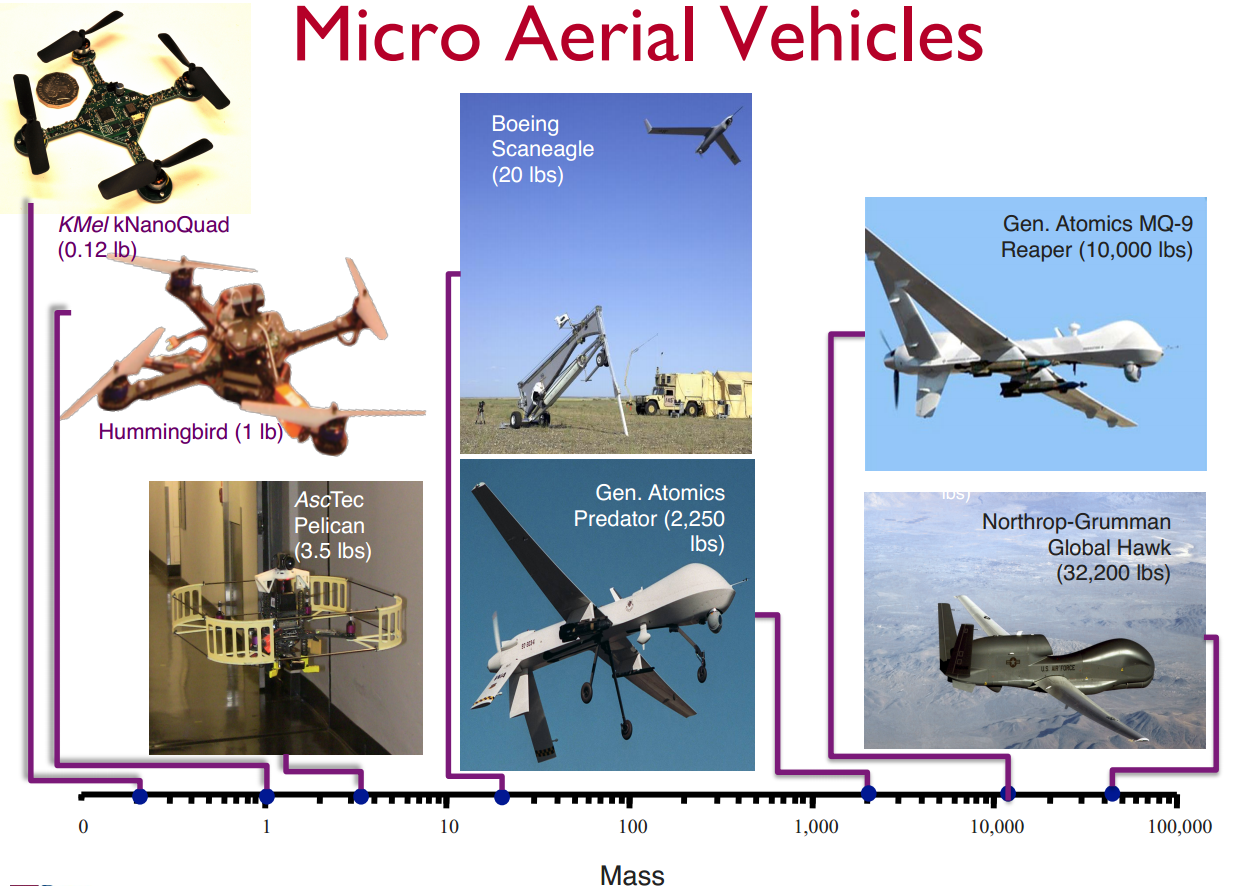
\includegraphics[width=\linewidth]{figures/Micro_aerial.png}
  \caption{Micro aerial vehicle}\label{fig:micro_aerial} \cite{Ardrone2}
  \endminipage\hfill
\end{figure}

The figure \ref{fig:micro_aerial}  shows some of the current UAVs. From cheap and small toys that you can be bought anywhere as the RC planes, toy quadcopter, to big military projects such as the Global Hawk. 

UAVs have recently found decline in their cost especially the quadcopters. In this thesis during the practical implementation part, quadcopters as one type of the rotor crafts will be used. The quadcopter used is Ar.drone 2.0 from the french company parrot. It is offshelf drone that can be found in market with comparable cheap price in range of 300 euros depending on the extras. It has been used several times in research labs and studied in \cite{Ardrone1},\cite{Ardrone2},etc.

There are many advantages that makes quadcopter as specific type of UAVs, suitable for both indoor and outdoor applications. It takes off vertically, do not need a runway, hover in its place, comparably light weight, and small in size.

For simulation V-REP with a model of quadcopter available was used. Some modification in this model was introduced to cope with the problem being solved and will be discussed later in more details. In both the practical work and simulation, ROS packages were used, tuned and implemented to control the quadcopter.

% There was no embedded systems work done and offshelf usage of the drone was utilized.

Some of the previously mentioned applications require area coverage of outdoor or indoor mapping. Coverage path planning is an active research topic as sub division of the general path planning problem that is studied by robotics domain for several decades till our day. It has been applied on many platforms in many areas where these platforms work. Normally the area to be covered is not a regular one. Most of the literature review that come to the awareness to the author of this thesis are concerned with uniform areas and prior map with static or dynamic obstacles in it. Platforms here means the mobile robots like autonomous underwater vehicles(AUV), unmanned aerial vehicle(UAV), or ground vehicles. 

% Aerial robots is still under study, investigation and development because of the many constrains and challenges that are in software and hardware of its construction on  many levels and layers. 

Prior information about the environment is assumed to be given in the form of a rough map for the area required to be covered. For this work, we model the set of coverage problems as arc routing problems. Although these routing problems are generally NP-hard, our approach aims for optimal solutions through the use of low-complexity algorithms in a branch-and-bound framework when time permits and approximations when time restrictions apply.


The final objective of this thesis research is to design a global optimization scheme allowing a cameras network to be self organized or to plan single trajectory of a flying robot equipped with a camera, according to fixed priority and constraints, in order to ensure a full coverage of a given scene. Applicable solution for both indoor and outdoor with ensuring coverage of the terrain while minimizing path repetition. Then building a mosaicking of the area covered and compare it with the original scene.


% %\textcolor{davidS}
% {The main problem of UAVs is the autonomy of fly, because of the battery run-time. This short time action restrained the possibility to use a set of UAVs and the work cooperation for a long time surveillance if there is no much UAVs available at the moment}. One smarter possibility is to create a monitoring path with several UAVs which  %\textcolor{davidS}
% {alternately automatically relays when the battery is low.} 
% During the navigation of the UAV's path, it is possible to get the image of the area to survey and build the mosaic of the area. 
% This paper will focus on finding the best waypoints for the UAV to pass through, to reduce the computation usually done in the path planning and coverage process. In order to find a good path to cover most of the area the essential point is to propose the best waypoints. %Finding the waypoint can be reduced to the problem of finding the best coverage.

% ensures complete coverage of the terrain while minimizing path repetition indoor gps denied  slam methods were used to localize and navigate the UAV using the visual 

In the next subsection the objectives of this thesis will be discussed.

\subsection{Objectives}
\begin{itemize}

\item Study coverage path planning problem, implement the suitable one.
\item Test and validate the path planning in both simulation and real world with practical hardware.
\item Construct a final mosaicked scene after the UAV acquire images.

\end{itemize}

\subsection{Thesis Organization}

%\printglossaries
\chapter{Background} \label{chap:background}

% Boustrophedon cell decomposition based coverage method 
% not Boustrophedon area coverage from right to left and from left to right in alternate lines.
% veer the uav from the desired path

The merit of this thesis in the coverage path planning context is splitting and decoupling the process of the coverage problem. The process will consist of: finding the proper pose and orientation of camera views that maintain area coverage, then apply path planning techniques to traverse these poses. So that the first part can be used as a solution by itself with positioning cameras in the obtained positions. The second merit is minimizing the overlapping paths and implementing the path planning taking into account the footprint of the robot and the camera, not relying on the assumption of robot representation as a point. % here the footprint of the camera only not the robot too 

\section{Related Work in path planning}
\subsection{Coverage Path Planning}
There are two main surveys that this literature review is relying on in picking and comparing the path planning technique to be further implemented and tested on the quadcopter. These surveys are; a survey on coverage path planning for robotics \cite{CPP2}, and coverage for robotics survey of recent results\cite{CPP1}.

There are a lot of other work extensively explored from many research areas beside path planning like computer vision, and graph theory. The problem can be studied from many sides like mapping, searching, patrolling, and applications. We focus here about the path planning and area coverage problems with slightly different approach than the common one. we take into consideration the footprint of the camera and one of the goals is to reduce the number of waypoints with maximum area coverage. Full area coverage in terms of 100\% is not the constraint.

In the literature generally there is always a navigation pattern to pass through the whole space; the robot need to cover. This pattern is done after decomposing the map into either regular cells or irregular ones like Voronoi. These methods can be categorized as heuristic and approximate, partial-approximate and exact cellular decompositions as discussed in \cite{CPP1}.

Coverage algorithms can be classified as heuristic or complete depending on whether or not they provably guarantee complete coverage of the free space. At the same time, they can be classified as online or offline. Offline algorithms rely only on the stationary information, and the environment is assumed to be known. Usually online algorithms are needed if some kind of adaptivity to the environment is required. Online algorithms usually utilize real-time sensor measurements. Thus, these algorithms can also be called sensor-based coverage algorithms.

The heuristic approach that is based on random path which is like the one equipped in some lawn mower and vacuum cleaner robots as mentioned in \cite{CPP1} can not be considered for aerial robots applications. 
Coverage algorithms can rely on cellular decomposition with many techniques that an extensive comparison was given in \cite{CPP2}; then an ox plowing motions is used like the example in planning algorithm book \cite{planningBook}. As the approach used in this thesis will not rely on map decomposition, further investigation can be found in the cited papers and book. \textcolor{red}{ If not decomposition how to say grid decomposition } 


\textcolor{red}{These algorithm can result in redundant coverage.}

Other approaches like  Artificial Potential Fields (APF), graph algorithms and neural networks can be used instead of the map decomposition. \textcolor{red}{||||||}




\subsection{Coverage Path Planning for UAVs}
There are various ways to obtain the path planning and optimize them.
CPP problem is a sub-field of path planning and well studied for ground vehicles like cases in \cite{CPP1,CPP2,path_planning_UGV}.

\textbf{CPP for UAV in general} 

In operations research, the CPP problem represent the environment as a graph, and using algorithms such as the traveling salesman(TSP) or postman problems to generate optimal solutions. In the graph representation, locations in the environment is represented as nodes in the graph and the paths between the locations are the edges. Each edge has a cost assigned to it where the cost can represent measurements such as distance(Euclidean,Mahalanobis,etc) between locations, terrain traversability, travel time or a combination of several metrics. These edges can be constrained or unconstrained with directions. More precisely undirected , directed graphs.

Voronoi diagram is also another possible solution as developed in \cite{voronoi_UAV} for decomposing the desired area and find the feasible solution from the starting point to the goal point through two step path planning algorithm, but it doesn't take into consideration the repetition rate constraint or full area coverage. For these reasons considering the solution used for arc routing problem is most beneficial.

TSP considered one problem of a large class of problems known as combinatorial problems and introduced in UAV path planning for several purposes like refueling depots in \cite{TSP_UAV}, multiple UAV cooperative reconnaissance in \cite{TSP_UAV_Multi}. This is a non-deterministic polynomial-time hard (NP hard) problem, that is sub-optimally solvable by many approaches as found in various research fields \cite{TSP_NPHARD}. Evolutionary approaches specifically  will be considered in this thesis.  

\subsubsection*{Evolutionary algorithms}

% \textbf{In this thesis considering one UAV operation to solve the CPP problem using GA as global path planning followed by local path planning solution.} 

Evolutionary Algorithms(EA) as sub branch of meta-heuristic optimization algorithms, imitates the biological process of evolution in nature. There are various algorithms that are branched from it like Ant colony optimization (ACO), particle swarm optimization (PSO),Genetic Algorithm GA and many more which can be studied from \cite{Evo_Book1,Evo_Book2}. GA uses techniques of inheritances, mutations, selections and crossovers of chromosomes over several generations of possible solutions to find convergence to the most optimized solution. Explanation in the next chart is the general abstract view of GA, more details will be explained in the methodology chapters.

\tikzset{
  frame/.style={
    rectangle, draw, 
    text width=6em, text centered,
    minimum height=4em,drop shadow,fill=lime!40,
    rounded corners,
  },
  line/.style={
    draw, -latex',rounded corners=3mm,
  }
}

\begin{tikzpicture}[font=\small\sffamily\bfseries,very thick,node distance = 4cm]
\node [frame] (pop) {Population};
\node [above=2cm, left of=pop] (init) {Initialisation};
\node [below=2cm, left of=pop] (term) {Termination};
\node [frame, above=2cm, right of=pop] (parents)  {Parents};
\node [frame, below=2cm, right of=pop] (off)  {Offspring};

\path [line] (parents)
 -- node[right,align=left,pos=.5] {Cross-Over\\[3mm]Mutation}
 (off);
\path [line] (init) |- (pop.170);
\path [line] (pop.190) -| (term);
%tournament 
\path [line] (off) -| node[below,pos=.25, align=center] {Survivor\\ selection}(pop);
\path [line] (pop) |- node[above,pos=.75, align=center] {Parents\\ selection}(parents);
\end{tikzpicture}

\subsection{Hybrid Algorithms for path planning}

\textbf{A two-level approach to collision-free navigation, using
artificial potential fields on the local lower solution planning, and GA solution to waypoints optimization problem represented as TSP for global higher layer planning}. 

then point-to-point motion planning problem, where the vehicle task is to navigate from a pre-specified initial point in the workspace to a pre-specified destination goal point.

\section{Waypoints Selection}

Finding the waypoints to have the best coverage of the area is close to the problem of positioning cameras or sensors to cover an area efficiently. Sensor positioning problem has been investigated since a few decades, mainly for video surveillance \cite{c1}. Without any additional constraint, this problem is NP-Hard as stated in \cite{c1,c2,c3,c4,c5} for the Watchman Route Problem (which is very similar to the optimal positioning waypoint for UAV path). Two non-optimal solutions have been proposed. The first one is based on Art Gallery Problem (AGP) \cite{c2,c3} and the second one is based on the Wireless Sensors Networks \cite{c6,c7,c8,c9} trying to find the best position to design an efficient network which can collect data with any kind of sensors. 

% do you mean here the the sensor pose is the most adequate solution

However, the solution proposed to the problem addressed the coverage problem but linked with additional and specific constraints, which are out of our scope. 
% like basic room without obstacles or focus on selection among the different possible sensor poses, which is the most adequate solutions. 
% This will become finding a solution among a set of more efficient subset of solutions, not a problem of finding a solution
%This will not become a problem of finding a position but to select among the set of more efficient subset of solutions. %or select the position sensor in the set of possible and restrained position
 %\cite{c7}.
 
 One of the algorithm used is the Particle Swarm Optimization (PSO) as detailed in \cite{c10,c11}. Zhou \textit{et al.} \cite{c10}, some experimental results are provided and one solution running in real time is proposed. However, the scene used in these experiments is rather small and many cameras are employed to fully cover it.  On the other hand, \cite{c11} uses a cost function but the cost function is not only focused on the position for surveillance and coverage, but also handling resolution and lighting, which affect the final solution by not covering the under illuminated areas.Reddy \textit{et al}. \cite{c11} also introduced the concept of “acceptable response”, allowing non-optimal/sub-optimal solutions. If the coverage score is higher than a given threshold, the solution is accepted and not locked by the research of an optimal solution. 
% Inspired by \cite{c10,c11}, extending the method for UAV waypoints positioning and path planning in more complex environments (basic room, big room, non-square shape).
 
 \section{UAV Localization} \label{localization_Back}
 
UAV localization problem is the challenge of finding the pose in terms of position and orientation of the aerial robot with reference frame. This reference frame can be with the initial point the robot is launched from, or a point in the map. There are two main categories for localizing the robot; either indoor or outdoor. For outdoor, GPS based navigation system is often used to determine the UAV’s absolute position. Also equipped with inertial measurement unit (IMU), UAV's orientation and acceleration can be estimated. State estimation of the UAV is obtained by coupling the previous obtained data with the UAV's mathematical model. This information is essential for autonomous navigation and of significant importance to aid the pilot to achieve smoother navigation. \textbf{Unlike ground vehicles, just holding the robot's pose requires values to withstand its place , giving order continuously to the robot   This is particularly the case for an aerial vehicle - while for ground-based vehicles not moving typically is a trivial task, this is not the case for a flying robot. Holding a position in the air requires constantly counteracting minor randomly induced movements, which in turn requires a method to detect these movements.}.
While for indoor localization challenge employing the IMU data can provide relative location, over time small errors will keep accumulating and drift will happen and affect the localization. Additional information about global positioning should be available to recover for this drift using means of filtering and sensor fusion \textbf{CITE} 

 This method will not be feasible when flying indoors where there is no reliable or cheaply available GPS modules available - alternative localization methods are required. For these reasons a solution  relying only on the UAV's sensors, using external tracking devices or external fiducial markers tracked by onboard camera. \textbf{CITE} 
 

An example of the available external tracking device are motion capture cameras that allow the robot to measure its position with very high precision and accuracy as in \cite{michael2010grasp}. Reflective markers like retroreflective dots attached to the robot, the cameras can estimate the position of each reflective marker and these cameras can do it at split second timing exceeding speeds of 100-200 times a second. This system will not be used as it requires setup up of several cameras which cost dozens of thousands of euros. The other external solution provided for example in  \cite{meier2012pixhawk} using external markers and detected using onboard camera. This solution could have been considered, but it is not the chosen one to be implemented in this thesis. 
 
 
 There are wide range of sensors can be equipped on the UAV to be help its localization like laser range scanner, monocular camera, stereo camera, RGB-D sensor, or ultrasonic range sensors. The usage of monocular camera is chosen to be the solution for this thesis. They provide competitive advantages; as they are cheap, energy-efficient, small and light. \textbf{CITE} Simultaneous localization and mapping (SLAM) can be achieved by combining visual pose estimates from the monocular camera  with additional sensor measurements available like the implementation of Tardif et al. in \cite{tardif2008monocular}. The tool developed by the computer vision group in Technical University of Munich as mentioned in the papers \cite{engel14ras,engel12iros}, is utilized on an AR.Drone 2.0 available in the lab with minor modification and plugin suitable to the specific coverage problem.
 
\section{Mosaicking}
without considering the features of the images, but relying on the given position and orientation. 
 
%  feature based : http://cseweb.ucsd.edu/classes/fa02/cse252c/smallick.pdf

%  comparison : http://citeseerx.ist.psu.edu/viewdoc/download?doi=10.1.1.677.1527&rep=rep1&type=pdf
\chapter{Optimized Waypoints Selection} \label{chap:optimizedway}


%%%%%%%%%%%%%%%%%%%%%%%%%%%%%%%%%%%%%%%%%%%%%%%%%%%%%%%%%%%%%%%%%%%%%%%%%%%%
%%%%%%%%%%%%%%%%%%%%%%%%coverage%%%%%%%%%%%%%%%%%%%%%%%%%%%%%%%%%%%%%%%%%%%%
%%%%%%%%%%%%%%%%%%%%%%%%%%%%%%%%%%%%%%%%%%%%%%%%%%%%%%%%%%%%%%%%%%%%%%%%%%%%
\section{Coverage}

\subsection {Context of experiment}

The main purpose of our work is to estimate the position of $n$ camera waypoints for surveying a given area in order to maximize the visual coverage. Each camera provides a top view of the area similar to UAV views. The coverage area of each camera is defined by the projection of the visual field onto the ground. This way, the mosaic composed of the captured images should be very close to a complete top view of the area. 
In order to find the best coverage, many experiments have been done to compare PSO and also GA. PSO is easier to implement and runs faster but GA is more flexible and generic thanks to the many tunable parameters. 
The following subsections will give an  overview our method, which is based on GA, and provide a comparison between PSO and GA that demonstrates the overall advantage of the latter on the former.

\subsection{ Cost function }

Since the goal is to maximize the visual coverage of the camera network, a cost function has been chosen to quantify it, as follows: 
\begin{equation}
 \sum_{i=1}^n = \frac{cover(i)}{size(grid)} _{1\leq i\leq n}  ,
\end{equation}
where $n$ is the number of waypoints; 
$grid$ represents the discretization of the ground plane (floor);
$cover($ ... $)$ is a function which computes the area on the ground which is covered by at least one camera ;
$size($...$)$ is the dimension of the full area which must be $covered (grid)$. 
% \begin{itemize}
% \item[-] Where $n$ is the number of cameras; 
% \item[-] $grid$ represents the discretization of the ground plane (floor);
% \item[-] $cover(…)$ is a function which computes the area on the ground which is covered by at least one camera ; %(see the pseudo-code below);
% \item[-] $size(…)$ is the dimension of the full area which must be $covered (grid)$. 
% \end{itemize}



\begin{figure}[!htb]
\minipage{0.40\textwidth}
  \includegraphics[width=\linewidth]{figures/Camera.jpg}
  \caption{Projection of the camera on the ground.}\label{fig:cam_proj}
  \endminipage\hfill
\end{figure}

Camera projection model is not explicitly taken into account, but the ground-projected visual field instead, as described in Fig.\ref{fig:cam_proj}.

%\includegraphics[width=0.3\textwidth]{Camera.jpg}
%\caption{Projection of the camera on the ground}
\subsection{Genetic algorithm }
Motivated by Darwin's theory of evolution and the concept of “survival of the fittest”, GAs use processes analogous to genetic recombination and mutation to promote the evolution of a population that best satisfies a predefined goal [12]. Such kind of algorithms requires the definition of a “genetic representation” of the problem and of a cost function used to evaluate the solution. The candidate solution is represented by a data structure named chromosome, defined by Eq.(\ref{Eq:xyzteta}) with $x,y$ and $z$ the cartesian coordinates and $\theta$ the rotation of the camera with respect to the optical axis: only  two possible angles are allowed, 0$^{\circ}$  or 90$^{\circ}$ (portrait or landscape). To pass from an iteration (or generation) to the other a few steps are necessary (see Fig.\ref{fig:GAexp}).
\begin{equation}\label{Eq:xyzteta}
     A=\begin{bmatrix}
         X_{i} \\
         Y_{i} \\
         Z_{i}\\
         \theta_{i}
        \end{bmatrix}_{1 \leq i \leq n}
  \end{equation}

\begin{figure}[t]
\minipage{0.95\textwidth}
  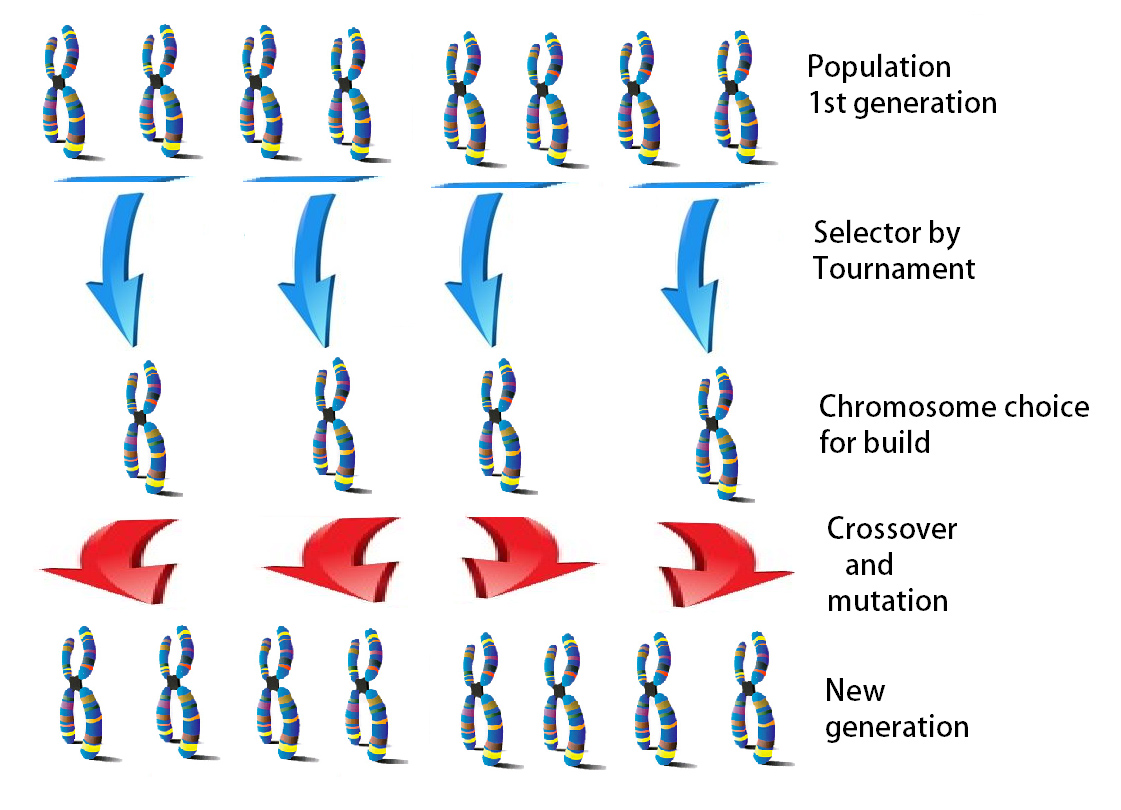
\includegraphics[width=\linewidth]{figures/GAfinal.jpg}
  \caption{ GA explanation, from one generation to the other.}\label{fig:GAexp}
  \endminipage\hfill
\end{figure}
In our experiments, we empirically fixed %after having sevral test in difrent condition the solution shosen is
the number of chromosomes to be 90, the mutation rate to be 0.001 and the crossover rate to be 0.919. 

\subsection{ Context of experimentation }

In order to compare the two algorithms and evaluate their performances, we tested them on different scenarios depicted in Fig.\ref{fig:Rooms_shapes}, with areas  of different sizes and shapes, where: 

\begin{figure}[!htb]
  \centering
  \hspace*{\fill}
  \subfigure[]{\label{subfig:r1}\includegraphics[width=0.45\linewidth]{figures/Room1.png}} \hfill
  \subfigure[]{\label{subfig:r3}\includegraphics[width=0.45\linewidth]{figures/room3.png}}
  \hspace*{\fill}
  \\
  \hspace*{\fill}
  \subfigure[]{\label{subfig:r2}\includegraphics[width=0.45\linewidth]{figures/room2.png}} \hfill
  \subfigure[]{\label{subfig:r4}\includegraphics[width=0.45\linewidth]{figures/room4.png}}
  \hspace*{\fill}
  \\
   \hspace*{\fill}
  \subfigure[]{\label{subfig:r5}\includegraphics[width=0.45\linewidth]{figures/room5.png}}
  \hspace*{\fill}
  \caption{Scenarios used for the experiments: (a), (b), (c) are   with z=1 and (d), (e) with z=2. The gray rectangle represents the field of view of one camera projected onto the ground.}
  \label{fig:Rooms_shapes}
\end{figure}

% \begin{figure}[!htb]
% \minipage{0.47\textwidth}
%   \includegraphics[width=\linewidth]{Room1.png} 
%   \label{fig:room1}    (a) 

% \endminipage\hfill 
%   \minipage{0.47\textwidth}
%   \includegraphics[width=\linewidth]{room3.png}  
%   \label{fig:room1}  (b)

%   \endminipage\hfill 
%   \minipage{0.47\textwidth}
%   \includegraphics[width=\linewidth]{room2.png}  
%   \label{fig:room1}  (c)
%   \endminipage\hfill 
%   \minipage{0.47\textwidth}
%   \includegraphics[width=\linewidth]{room4.png} 
%   \label{fig:room4}  (d)
%   \endminipage\hfill  
%   \minipage{0.47\textwidth}
%    \includegraphics[width=\linewidth]{room5.png}
%    (e)\label{fig:room1}  
 
%  \caption{Scenarios used for the experiments: (a), (b), (c) are   with z=1 and (d), (e) with z=2. The gray rectangle represents the field of view of one camera projected onto the ground.}
%   \label{fig:Rooms_shapes}  
%   \endminipage 
% \end{figure}

% In order to compare the two algorithms and evaluate their performances, we tested them on different scenarios depicted in Fig.\ref{fig:Rooms_shapes}, with areas  of different sizes and shapes, where: 
	
\begin{itemize}
\item[-]    z is the height of the camera between (within the range $[1⁄/z;z]$).
\item[-]	Figure~\ref{subfig:r1} is an area of size 120$\times$80 (named Room). 
\item[-]	Figure~\ref{subfig:r2} is an area of size 240$\times$160 (named Big room)
\item[-]	Figure~\ref{subfig:r3} is an area of size 120$\times$80 (named Room U)
\item[-]	Figure~\ref{subfig:r4} is an area of size 120$\times$80 (named Room L)
\item[-]	Figure~\ref{subfig:r5} is an area of size 240$\times$80 (named Big room L)
\end{itemize}


% \begin{figure}[!htb]
% \minipage{0.72\textwidth}
%   \includegraphics[width=\linewidth]{roomsize.png}
%   \caption{Scenarios used for the experiments: (a), (b), (c) are   with z=1 and (d), (e) with z=2. The grey rectangle represents the field of view of one camera projected onto the ground.}\label{fig:Rooms_shapes}
%   \endminipage\hfill
% \end{figure}



The design of experiments in Table \ref{table:table1} has been set up to identify the most efficient algorithm for the positioning of a set of waypoints with the maximum of coverage. 

%\hfill

%% tablo  designe of experiment
\begin{table}[!htb]
\begin{tabular}{|l|l|l|l|l|l|}
  \hline
  \multicolumn{2}{|l|}{z=1 } &\multicolumn{2}{|c|}{GA}  & \multicolumn{2}{|c|}{PSO} \\  \hline
  \multicolumn{2}{|c|}{ } & GT & NW & GT & NW\\ \hline
  Room &  120x80 & 16 &20 & 16 & 20\\ \cline{2-6}
     &  240x160 & 64 &70 & 64 & 70 \\ \hline
  Room U &  120x80 & 12 &20 & 12 & 20\\ \hline
  \multicolumn{2}{|l|}{z=2 } &\multicolumn{2}{|c|}{GA}  & \multicolumn{2}{|c|}{PSO} \\  \hline
 Room &  120x80 & 4 &10 & 4 & 10\\ \cline{2-6}
     &  240x160 & 16 &20 & 16 & 20 \\ \hline
 Room L&  120x80 & 3 &10 & 3 & 10\\ \cline{2-6}
     &  240x160 & 15 &20 & 15 & 20 \\ \hline
\end{tabular}
\caption{Design of experiment for compare the efficiency of PSO and GA in different condition.  (GT is Ground Truth and NW is Number of Waypoints).}\label{table:table1}
\end{table}
The Ground Truth (GT) is the minimum number of waypoints required to fully cover a given area. The size of the area has been selected so that the GT can be easily estimated. NW is the maximum number of waypoints (or camera views) used for the experiments. At each experiment a solution is computed for a number of waypoints from 1 to NW. In order to compare the different algorithms in similar conditions, only 10000 calls of the cost function is allowed for each set of waypoints.

\subsection{ Analysis of the result}
After performing the design of experiments (see Table \ref{table:table1}) it appears that GA and PSO algorithms are close in performance. In some cases GA is much more efficient (see in Fig.\ref{fig:bigRz1}) particularly in the case where the search space is large (big room and high number of cameras)  as example in Fig.\ref{fig:bigRz1}). Instead, PSO is more effective to optimize small areas (see in Fig. \ref{fig:RLz2} ).
This efficiency can be explained by the small variation of the solution introduced by the PSO. 

However, this small variation is not enough to find an optimized solution in a big search space which happens when a lot of cameras are required or when the local minima is deeper. Although the variety of solutions introduced by the GA allow escaping from local minima, it can affect negatively the accuracy of the solution, which may require a further optimization step to refine. 

% and the solution proposed is less adjusted may have more difficulties to the adjusted to have a finer positions of any cameras and then the adjustment of positions is less precise.

%if the accurate and thorough optimization is more difficult, it is because the GA introduce lot of variety. 

%it takes longer time to get the most optimal solution 


\begin{figure}[!htb]
\minipage{0.62\textwidth}
  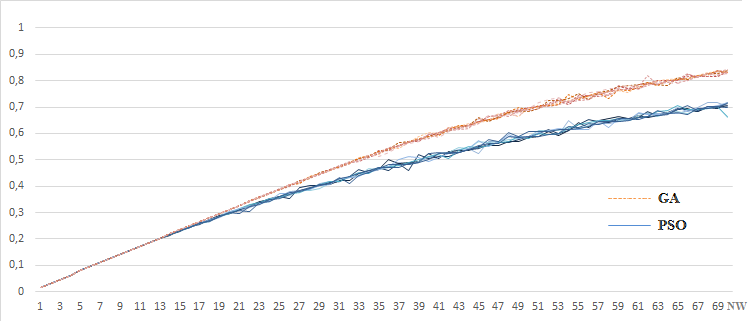
\includegraphics[width=\linewidth]{figures/GAPSObigRoomz1ters.png}
  \caption{ Comparison of  eight solution given by GA,  eight solution given by PSO algorithms with a Z equal to 1, in the big room 240x160 and ground truth equal to 64.}\label{fig:bigRz1}
   \endminipage\hfill
\end{figure}

\vfill
\hfill

\begin{figure}[!htb]
\minipage{0.62\textwidth}
  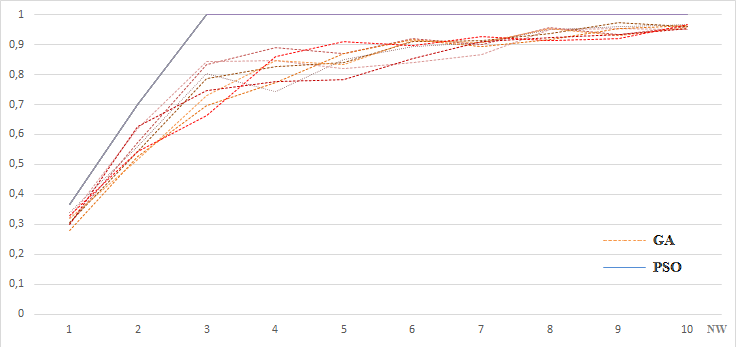
\includegraphics[width=\linewidth]{figures/GAPSORoomLz2bis.png}
  \caption{Comparison of eight solutions given by GA, eight solutions given by PSO algorithms with a Z between [1/2; 2], in the room with L shape 120x80 and ground truth equal to 15.}\label{fig:RLz2}
   \endminipage\hfill
\end{figure}

\hfill 
\vfill
\newpage

Following the comparison of the 2 algorithms, the GA seems more suited to find UAV waypoints especially if it navigates in a large room or outdoor scene. Furthermore, the comparative study demonstrated that the GA is less dependent on the shape of the  covered area. 


The number of UAV waypoints (camera pose) must be priorly known when using GA: the number of camera views is an input of the algorithm. However, in our application, it is far more interesting to assess the number of views with respect to the desired coverage rate of the area. 
To do so, a two-step procedure has been implemented. 
The first step is to find the minimum number of waypoints depending on the area to cover like  formulated in the Eq.(\ref{Eq:waypointN}). \\
\begin{equation}\label{Eq:waypointN}
\frac{ A_{room} - \sum_{i=1}^n A_{wall i} }{A_{cam}} \times \mbox{Threshold Rate} = \mbox{NWayPoint}
\end{equation}

\begin{itemize}
\item[-] $ A_{room}: $  area of the Room (length $\times$ width)
\item[-] $ A_{Wall}: $  area of the obstacle like wall (length $\times$ width)
\item[-] $ A_{Cam}: $   area cover by the camera in the maximum size of z
\item[-] $ \mbox{NWayPoint}: $  number of waypoints
\item[-] $ \mbox{Threshold Rate}: $ objective threshold rate 
\item[-] $S:$ one solution of waypoints set 
\item[-] $evalCost:$ cost function  
\end{itemize}

The second step is to compute GA optimization until the threshold is reached, while increasing the number of waypoints like explained in the algorithm \ref{alg:euclid}.  

\begin{algorithm}
\caption{}\label{alg:euclid}
\begin{algorithmic}[1]
\Procedure{N}{$a$}
 \State $S\gets 0$
  \While{$eval Cost(S)\leq ThresholdRate$}
	 \State $S \gets GA(NWayPoint)$
	  \State $NWayPoint\gets NWayPoint+1$
  \EndWhile\label{endwhile}
\State \textbf{return} $NWayPoint$
\EndProcedure
\end{algorithmic}
\end{algorithm}
\chapter{Optimized Path Planning} \label{chap:trial}
\iffalse
Keywords : 
Smooth Tour Construction with kinematic constrains,Dubins TSP,
Bezier Curve , cubic spline interpolation

bezier curve:
% http://www.joics.com/publishedpapers/2011_8_12_2441_2450.pdf

http://www.ijsce.org/attachments/File/v3i2/B1421053213.pdf
good explanation but it doesnt formulate as TSP . so refer to the book of planning and motion of UAV.


Global planner, local planner can be found  in lecture 10 planning of visual navigation for flying robots .. slide 79 before and after
The approach provided in this thesis is 2 layers of path planning. The first one is the global path planning where  the waypoints are sorted based on the shortest distance covered traversing all the given waypoints. The second layer is finding the paths between intermediate waypoints. 
This second layer can
\fi

As mentioned earlier in the previous chapter, the best waypoints to be traversed guaranteeing area coverage were chosen. Path planning algorithm should be implemented afterward to sort these waypoints in order to assure minimal traversal 3D euclidean distance. After sorting the waypoints, there are several methods to achieve the trajectory planning that the robot should follow in between them.

These processes of sorting the waypoints, then traversing in-between them;  can be formally explained as 2 layer path planning consisting of; global and local planners. Autonomous navigation of an aerial robot based on the combination of evolutionary algorithms as a global planner. Followed by one choice of the approaches discussed in section \ref{local_path_planning} as a local planner. These approaches can be summed up as a linear piecewise function, spline piecewise function and artificial potential fields.


% The hybrid approach first uses Grid Method where the robot environment is represented by orderly numbered grids, each of which represents a location in the environment. Then, it applies Genetic Algorithm (GA), a global planner, to find an optimal path according to the current environment. The GA proposed here uses an evolutionary population initialization and genetic operators, which make the evolutionary process converge after some populations. Finally, a new Artificial Potential Field method, a local planner, is applied to follow the path obtained by GA from one intermediate node to next intermediate node avoiding the obstacles. Experimental results clearly illustrate that the proposed hybrid approach works well on large scale dynamic environments.


%\textcolor{red} { hybrid PF with GA, 
%http://download.springer.com/static/pdf/746/chp%253A10.1007%252F978-94-007-2792-2_31.pdf?originUrl=http%3A%2F%2Flink.springer.com%2Fchapter%2F10.1007%2F978-94-007-2792-2_31&token2=exp=1463649025~acl=%2Fstatic%2Fpdf%2F746%2Fchp%25253A10.1007%25252F978-94-007-2792-2_31.pdf%3ForiginUrl%3Dhttp%253A%252F%252Flink.springer.com%252Fchapter%252F10.1007%252F978-94-007-2792-2_31*~hmac=ec049bb412555489f79488635013bb217387263b0f56bf6ea86e6e0965c82648
%}


Normally path planning optimization techniques does not put the constraint of passing by the defined waypoints as a hard constraint in their solutions. But rather, tend to change the waypoints depending on the robot motion in relative to the environment. In this thesis's case hard constrains of passing by the waypoins are taken into account. A global path planner is good in producing a minimal distance path, but poor in finding intermediate waypoints and reacting to unknown obstacle.

%\textcolor{red}{rectilinear environment}
%so we can not rely on cell decomposition % page 7 paper carera 

\section{Global Path Planning } \label{global_path_planning}
There are several ways to globally solve and find the robot path within a map. % lazem te3mel 7esab el map di hatnail fiha eh !! 

%formulate this problem. In this Thesis, two methods have been implemented and compared.

Some operations research methods, such as traveling salesman problem (TSP), Chinese postman problem and rural postman problem can be considered. In this thesis; TSP was taken into account. 


\subsection{Problem Formulation}


% The list of waypoints needs now to be sorted to compute an efficient path with smoother shape and shorter traveling distance. 

% \iffalse
% A process of using Dijkstra to compute an ordered list of waypoints providing shorter path. These waypoints in the sorted list is dealt with as temporary goals for the UAV to pass through. The next step is to fit the trajectory of the UAV as in \cite{curve_path}. For this waypoints are dealt as if they are graph nodes and transform the problem to be a linear or spline piecewise function .  
% \fi
% A process of formulating the problem of shortest path as traveling sales man problem and finding optimized solution using genetic algorithm is approached previously many times \textcolor{red}{citation} and validated its working principle, so it is used here in this context. The path output as ordered list of poses that guarantee the shortest path. The next step is to fit the trajectory of the UAV as in \cite{curve_path}. For this waypoints are dealt as if they are graph nodes and transform the problem to be a linear or spline piecewise function.


\subsubsection{Search Based Shortest Path Problem}
The goal of this category of methods is to find a continuous curve (no need to be smooth) in a configuration space that begins from the start node $x_{init}$ to the goal end node $x_{goal}$. It is mature enough method in research field with several algorithms like Dijkstra, A*, D*, and many more. % as discussed in the background 

%In our case we assume every waypoint as a goal, which define the problem as multi-goal Dijkstra path planning problem. The robot will search within its neighbour nodes for the node generating shortest path to every goal.
Representing the waypoints chosen previously as a weighted graph. The nodes of the graph are the waypoints, vertexes are an intermediate path between waypoints. The weights of the vertices are the Euclidean distances between waypoints. Dijkstra is then implemented to find the minimum cost path.

 %Dijkstra in this method will simply find at every iteration the waypoint with the shortest euclidean distance from the current waypoint. Traversed waypoint will be excluded at every iteration. At the end of this process a list of ranked waypoints with the least 3D euclidean distance between every waypoint and its succedent one is obtained. This will not guarantee a globally shortest distance path.
 Iteratively, Dijkstra will start from the initial node and search within the connected nodes for the one with the least weight. Choose this node to be its next initial node and repeat the process till all the required nodes are traversed and ranked.

%\textcolor{red}{write in algo Sora kaman momken}

%transform the area to be covered to a graph % transform the area to grid with discretize the graph up to a resolution needed  assign each pose as a node in the graph assign 3D Euclidean distance as the weight of the vertex between the nodes.

It is wide known of its slowness in the topological representation. The resolution and amount of waypoints considered as goals lead to very slow and nonoptimal convergence for passing by all these waypoints, so another formulation is required to be tested. The formulation discussed in the next section shows promising results.

\subsubsection{Traveling Sales Man Problem }
The robot traversing the waypoints can be formulated as traveling sales man problem(TSP). The TSP can be shortly explained as a salesman has to visit several cities (or road junctions). The goal is to find the salesman's route of minimum length with the constrain of passing by by all the cities only once. Mathematically modeling the problem as a complete graph with n vertices, the salesman will make a tour or hamiltonian cycle  \cite{dantzig1954solution}.

Sorting the path can be addressed as an optimization problem. Every node which is a point in space (3D position) is represented as a city and the euclidean distances between the cities are calculated and used as the optimization cost function. The path is organized based on the minimum length of traversing over all the waypoints. To find an optimized solution GA is used. The privilege of TSP problem formulation and solving it using GA over the other shortest path algorithms like Dijkstra, is that it provides global complete solution traversing all the waypoints not finding a path from a starting node to a goal node. The GA approach for multiple waypoint path planning is more clarified and discussed by Trevor \textit{et al.} in \cite{davies2006multiple}.


GAs generally consist of three operators: selection, crossover, and mutation. The evaluation function for the N cities two-dimensional Euclidean TSP is the sum of Euclidean distances between every pair of cities in the tour. 

That is: 
\[Cost function = \sum_{i=1}^{N}  \sqrt{(x_{i}-x_{i-1})^{2}+(y_{i}-y_{i-1})^{2}} \]
                                           
Where, $x_{i}$, $y_{i}$  are the coordinates of city i and  $x_{N}$, $y_{N}$   equals $x_{0}$, $y_{0}$. %We also make some changes to the encoding, selection, and recombination.

The algorithm can be explained in abstract as :
%\textcolor{red}{|||||||||||||||||}

%1. Generate a new population of the previous population by updating all paths in the current population. The point hereditary is determined. The path is amended by deleting the initial points and adding other segments to reach all paths to the end point.\\
%2. Start the algorithm for a static planning to the population and find the best path.\\
%3. Send the best path to the aerial robot when it reached the crossing point current.\\
%4. Update estimates of site locations for the environment.\\
%5. Go back to step one.\\

% REF : https://www.cs.indiana.edu/~vgucht/Genetic_Algorithms_for_the_Travelling_Salesman+Problem.pdf
% http://www.obitko.com/tutorials/genetic-algorithms/tsp-example.php
% http://www.ijsce.org/attachments/File/v3i2/B1514053213.pdf
%Algorithm 2 Genetic Algorithm

%1. Start
%2. Population initialization
%3. Repeat until satisfying stop criteria
%4. Selection
%5. Cross-over: two selected chromosomes can be combined by a cross-over operator, the result of which will replace the lowest fitness chromosome in the population. Selection of each chromosome is performed by an algorithm to ensure that the selection probability is proportional to the fitness of the chromosome. A new chromosome has the chance to be better than the replaced one. The process is oriented towards the sub-regions of the search space, where an optimal solution is supposed to exist.
%6. Mutation: a gene from the selected chromosome is randomly changed. This provides additional chances of entering unexplored sub-regions. Finally, the evolution is stopped when either the goal is reached or a maximum CPU time is reached.
%7. Making new population with the fittest solutions
%8. Evaluation
%9. Checking the stop criteria
%10. Take the best solution as output
%11. End

% http://www.lalena.com/AI/Tsp/
% http://www.theprojectspot.com/tutorial-post/applying-a-genetic-algorithm-to-the-travelling-salesman-problem/5

\begin{enumerate}
\item Create a group of many random tours in what is called a population. This algorithm uses a greedy initial population that gives preference to linking cities that are close to each other.
\item Pick two of the shortest tours which represent better parents in the population and combine them to make 2 new child tours. Hopefully, these children tour will be better than either parent.
\item A small percentage of the time, the child tours are mutated. Mutation of a tour is done by multiple ways like shuffling or swapping the route. Shuffling the route is done by randomly moving one of the cities from one point in the tour to another. Mutation is done to prevent all tours in the population from looking identical.
\item Crossover is done by picking two parents. Then take subset from the first parent and complete the child formation from the second parent.
\item The new children tours are inserted into the population replacing a number of the longest tours. The size of the population remains the same in every generation.
\item New children tours are repeatedly created until the desired goal is reached.
\end{enumerate} 


%\textcolor{red}{see the 3 dimentional part !! change in the code to adapt and then change the passage }



%B. The Algorithm GA
%1. randomly initialize population(t)
%2. determine fitness of population(t)
%3. repeat
%  1. select parents from population(t)
%  2. perform crossover on parents creating
%  population(t+1)
%  3. perform mutation of population(t+1)
%  4. determine fitness of population(t+1)
%4. until best individual is good enough 
%
%\begin{algorithm}
%\caption{}\label{alg:euclid}
%\begin{algorithmic}[1]
%\Procedure{N}{$a$}
% \State $S\gets 0$
%  \While{$eval Cost(S)\leq ThresholdRate$}
%	 \State $S \gets GA(NWayPoint)$
%	  \State $NWayPoint\gets NWayPoint+1$
%  \EndWhile\label{endwhile}
%\State \textbf{return} $NWayPoint$
%\EndProcedure
%\end{algorithmic}
%\end{algorithm}



% The privilege of GA over the Geometric Algorithms and sampling based algorithms is finding a complete solution traversing all the waypoints not finding a path from a starting node(pose) to a goal node(pose) %, not like grid or probabilistic methods used to navigate from one waypoint to another

% After having a sorted list of poses to be traversed, the next step is to fit the trajectory of the UAV as in Chang et al \cite{curve_path}.
\vfill

\begin{figure}[!h]
\minipage{0.53\textwidth}
  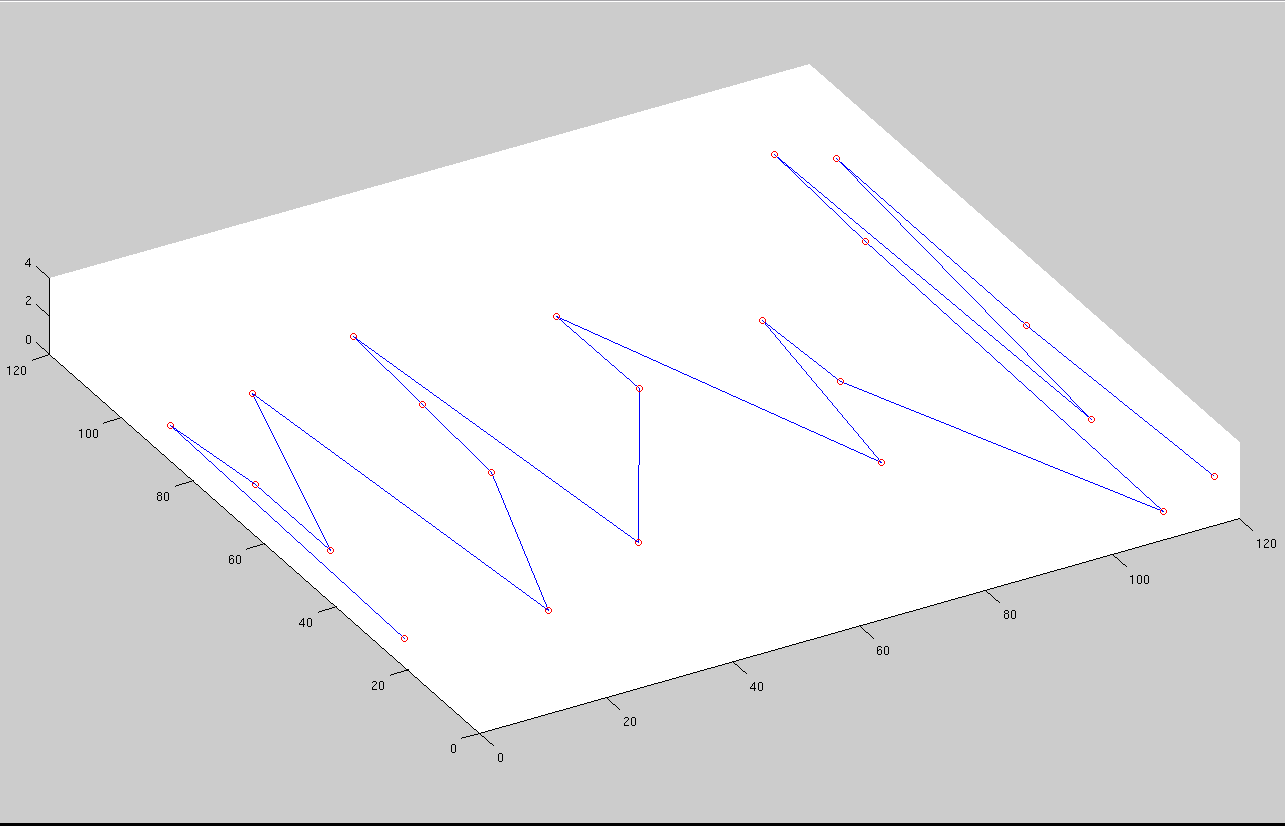
\includegraphics[width=\linewidth]{figures/DijkstraPath2.png}  
  \endminipage\hfill
  \minipage{0.45\textwidth}
   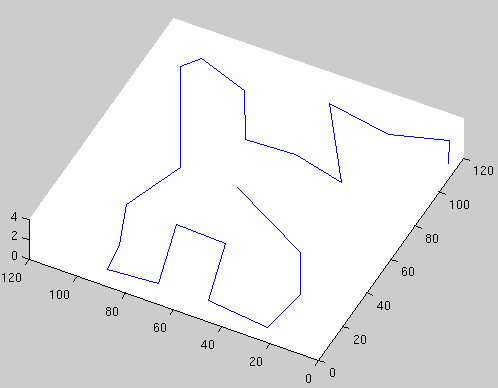
\includegraphics[width=\linewidth]{figures/Path_planned_G.png}
  \caption{Path using Dijkstra vs GA}
  \label{fig:Path_planning}
  
  \endminipage 
\end{figure}

%Traversing Distance was shorten by the 3.2 factor.  Before the path planning the distance traversed  was 166 meters and after GA applied it is nearly 51.3 meters 

The distance covered by a path that is planned by GA is 513 meters which is shorter by the factor of 1.8 compared to the distance covered by Dijsktra multi-goal approach which is 963 meters.


\section{Local Path Planning} \label{local_path_planning}

After succeeding in getting the main waypoints sorted in a way to grantee shortest path length. Forthwith comes the issue of generating the mid waypoints that the robot should traverse to generate the trajectory.

Three main ways have been implemented and tested. These ways will be mentioned in the next three subsections.

\subsection{Linear Piecewise Interpolation}
The previous process will provide a list of sorted  waypoints co-ordinates. These waypoints are dealt as graph nodes, that need to be connected to have a path, so the problem is formulated as a linear or spline piecewise function.

 Hereby the used linear piecewise function used in Eq.(\ref{eq:3}).

\begin{equation} \label{eq:3}
f(x)=
\left\lbrace
\begin{array}{ccc}
0  & \mbox{if} & x\leq a\\
\frac{x-a}{b-a} & \mbox{if} & a\leq x\leq b \\
\frac{c-x}{c-b} & \mbox{if} & b\leq x\leq c \\
1  & \mbox{if} & c\leq  x \\
\end{array}\right.  ,
\end{equation}

\noindent 
Where the line segment between points \textit{a} and \textit{b} will be the line between every waypoint and the consecutive one. The third point is \textit{c} and depending on the number of waypoints variables will be added in the formula. Discretizing this point up to an extent will act as the sampling the path. % to form a trajectory.


% \textcolor{red}{Shall i write the general equations of linear and spline piecewise fn. ?!}
% \textcolor{davidS}{????? i thing is more about ingeniery and implementation on robots }



\subsection{Spline Piecewise interpolation }
% for the equation : https://en.wikipedia.org/wiki/Spline_interpolation


% REF : http://www.math.colostate.edu/~gerhard/classes/331/lab/splines.html
% http://www.sciencedirect.com/science/article/pii/0736584589900458

% VERY IMPORTANT TO SIMPLIFY : http://citeseerx.ist.psu.edu/viewdoc/download?doi=10.1.1.713.6275&rep=rep1&type=pdf

% Field D*: http://robots.stanford.edu/isrr-papers/final/final-23.pdf

% https://www.youtube.com/watch?v=YtcZXlKbDJY

%spline length is shorter than polynomial interpolant

 The goal of the spline interpolation is to find the shortest smooth path through consecutive waypoints. This smoothness is advisable in order to eliminate the sudden change in the first derivative or the slope of the function (the line between the waypoints). It is very important as, robots specially aerial ones, require a portion of time and space to change direction and rotate. 
 
% Moreover, the discontinouity in the fist derivative of the poses (velocities); which are used in the low level control of the robot's motors .

% ‘spline’ - not-a-knot cubic spline interpolation

%length of the interpolant = \textcolor{red}{there is a way to calculate it check }

When the interpolation is assumed to be piecewise linear, it is relatively easy. However, if the curve is to be a spline, perhaps interpolated as a function of chordal arc length between the points, this gets a bit more difficult. A nice trick is to formulate the problem in terms of differential equations that describe the path along the curve. Then the interpolation can be done using an ordinary differential equation solver. For instance, the robot used in this thesis is a quadcopter; which is considered to be holonomic. Its kinematics give hovering capabilities. This feature permits to relax turning constraints on the path (which represents a crucial problem for fixed-wing vehicles).
The implemented interpolation as shown in the results section \ref{experiment_reuslts} is a cubic spline. This cubic spline of the $i^{th}$ spline function, in general, can be written as:
\begin{equation}
s_{i}(x)=a_{i}+b_{i}(x-x_{i})+c_{i}(x-x_{i})^2+d_{i}(x-x_{i})^3
\end{equation}
For n data points, there are n-1 intervals and thus 4(n-1) unknowns to evaluate to solve all the spline function coefficients. $a_{i}$, $b_{i}$, $c_{i}$, and $d_{i}$ must be determined for each \textit{i}. More investigation about spline interpolated path planning can be found in \cite{judd2001spline}.

% https://www.math.ohiou.edu/courses/math3600/lecture19.pdf

\subsection{Artificial Potential Field}
It was promising idea when Artificial Potential Field (APF) was first introduced in the robotics field by Oussama Khatib in 1986 \cite{khatib1986real}. With simple rules defined in the paper as a potential function between free space and obstacle space. The goal position to be reached is an attractive pole for the robot and obstacles are repulsive surfaces.

% stated The manipulator moves in a field of forces \textcolor{red}{explain more}. 

The procedure involves the following steps:
\begin{enumerate}
\item Establish a potential field function.
\item Locate a minimum potential point using any optimization algorithm.
\item Navigate an object toward the minimum potential point.
\item Repeat steps 2 and 3 until the object reaches the goal position.
\end{enumerate}

\begin{equation}
\begin{split}
U(q)=U_{att}(q)+U_{rep}(q) \\
U_{rep}(q)=\sum(U_{obstacles}(q))
\end{split}
\end{equation}

\begin{equation}
F(q)=-\nabla U(q)
\end{equation}
Where
$U_{att}$ is the attractive potential and
$U_{rep}$ is the repulsive potential. F(q) is the local force that will let the robot move by small steps.
There are various functions to model the potential field. The parabolic one is used in this context. 
Following an iterative gradient decent can be a simple way to go to the bottom where the goal point is available. 

\[q_{i+1}=q_{i}+\delta_{i}\frac{F(q)}{\left \| F(q) \right \|}\]


% online collision avoidance approach

As obstacle avoidance was the original goal of this algorithm, potential fields come with the risk of getting stuck in local minima and not being able to reach the goal. There are several solutions to this inherent characteristic. one of them is to methods like RRT to plan the path in the generated potential field map like what stated by Latombe et al. in \cite{latombe2012robot,planningBook}. In our specific case, the global path planner set the initial point and the goal point provided to the APF with a guarantee to have a short distance which should not lead to a local minimum. Here APF is tweaked to only avoid the obstacles that may appear in the map, not planning the whole path.
% parameters like the rotation and .... blbla has to be defined for the robot to navigate the whole map.
\section{Summary}

%\textcolor{red}{ the pathplanning book 3.5.2.2 GA PF}

\begin{figure}[H]

  \includegraphics[width=0.92\textwidth]{figures/main(1).png}
  \caption{Pipeline of the methodology}
  
  \label{fig:pipeline_1}  
\end{figure}
\chapter{Experiments and Results}

As mentioned earlier, the work presented in this thesis is prepared on simulation and validated on real micro UAV robot. More details about the environment of the simulation is found in \ref{simu}, and about the real robot in \ref{real_robot}. An abstraction for the real robot's hardware and software specifications are mentioned in \ref{real_robot_hardware}. Robotics Operating System (ROS) has been used because of its advantages that will be discussed in section \ref{ROS_part}.

\section{Robotics Operating System} \label{ROS_part}
In the past years ROS has proved its value and grown great attention in both research and industry since it is first introduced by Andrew Ng. et al. in 2009 \cite{quigley2009ros}. It is an open source message oriented middleware with publisher subscriber message passing process. Collaborators from many companies and research laboratories develop packages and tools with the concept of being reusable. 

% some are generic with no restriction of the hardware used. 


There are now mature enough tutorials, that can give extensive and deep view of ROS like for example technical books that show step by step development using ROS as in \cite{o2014gentle,joseph2015mastering}. 



\section{Simulation} \label{simu}
There are variety of robotics simulations available in the field nowadays like MORSE, Gazebo, V-REP,Stage, etc. Available comparison about can be found examined by Gonçalo Nuno in \cite{augusto2013robotteamsim}.
\vfill
\hfill
% Some applications that utilize ROS and V-REP environment in their research as in \cite{olivares2014v}

\subsection{VREP}
Virtual Robot Experimentation Platform (V-REP) is introduced in 2013 by E. Rohmer et al. in \cite{rohmer2013v}. It has great advantage in speeding up the process of algorithm's development visualization and validation. The robot simulator V-REP, model can be individually controlled via an embedded script, a plugin, a ROS node, a remote API client, or a custom solution. This makes V-REP very versatile and ideal for multi-robot applications. Controllers can be written in C/C++, Python, Matlab, and more.
\vfill
\hfill

\subsubsection{Room}

Several rooms were built in V-REP to act as different room scenarios.

\begin{figure}
  \centering
  \subfigure[Small Room]{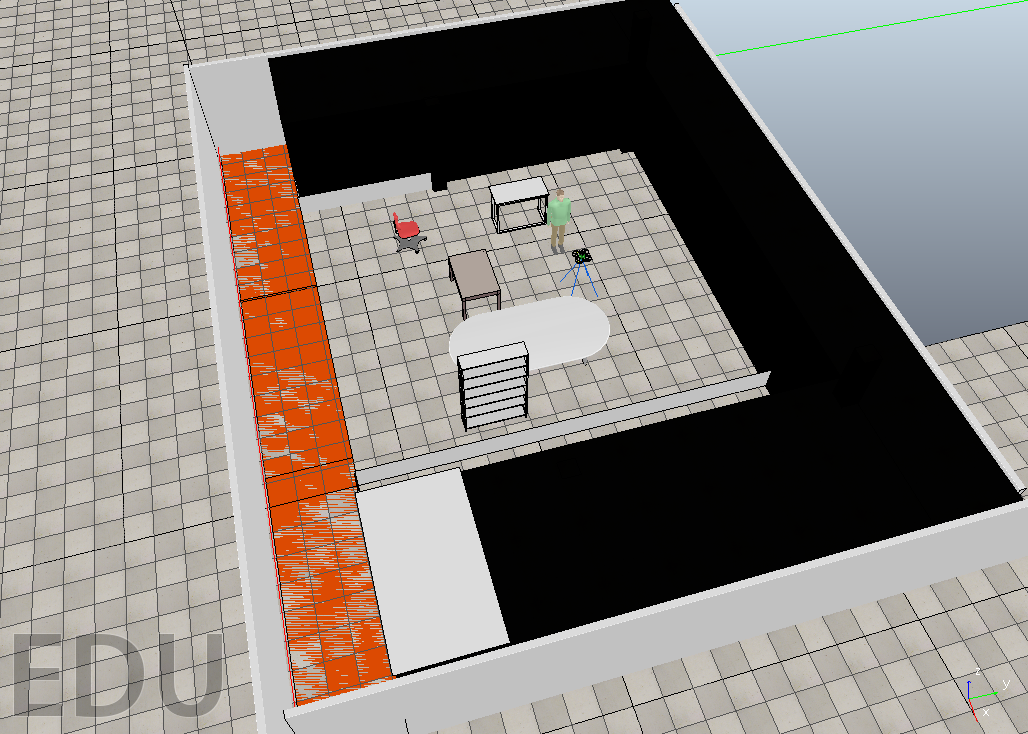
\includegraphics[width=0.45\textwidth]{figures/Room_2.png}}
  \hfill
  \subfigure[Big room]{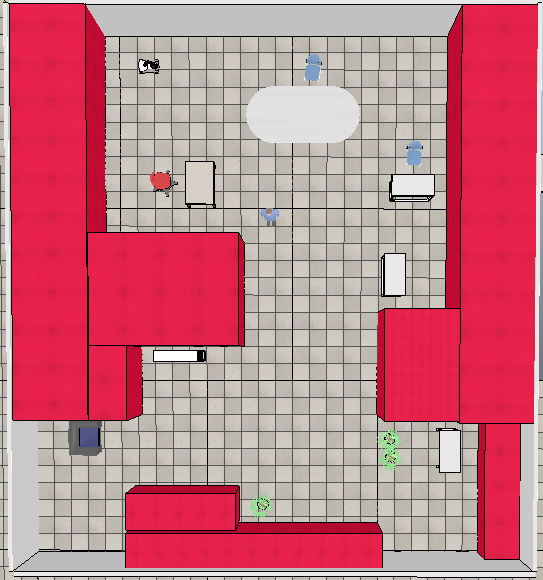
\includegraphics[width=0.45\textwidth]{figures/room_full.png}}
  \caption{Room Coverage}
  
  \label{fig:final_room}
\end{figure}

\vfill
\hfill

\subsection{UAV Simulation}
\begin{figure}[!]

  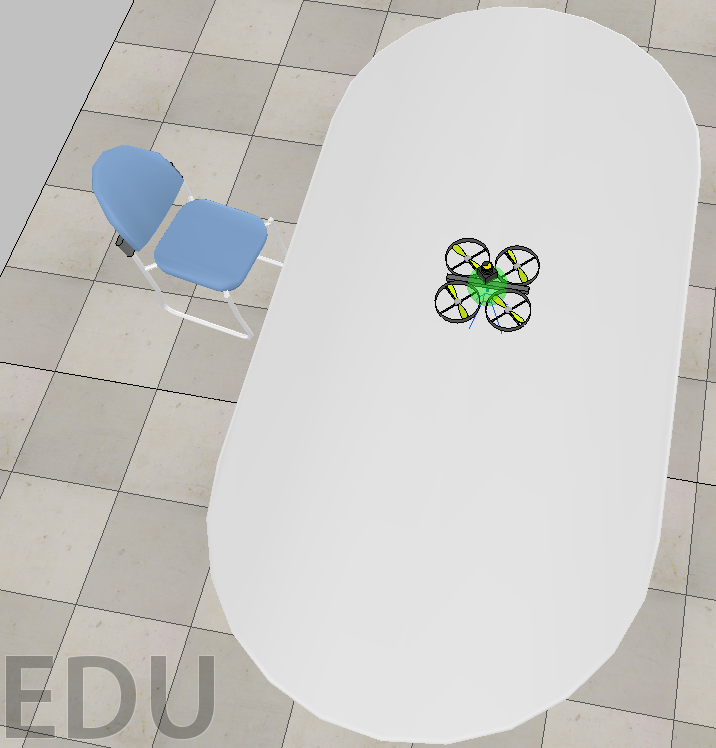
\includegraphics[width=0.5\textwidth]{figures/Drone_VREP.png}
  \caption{Drone available in V-REP with some modifications}
  
  \label{fig:drone_vrep}  
\end{figure}

\vfill
\hfill

\subsection{UAV model}

The UAV used either in simulation or real world experimentation is of micro aerial quadcopter drone like in figure \ref{fig:drone_vrep}. Obviously from the name comes quad which is equivalent to have 4 blade rotors. The quadcopter is controlled by adjusting the angular velocities of the rotors which are spun by electric motors. It has simpler structure compared to the other rotor crafts like helicopter. It can easily take off and land with vertical takeoff and landing (VTOL).  \textbf{CITE for more info}

% REF : http://sal.aalto.fi/publications/pdf-files/eluu11_public.pdf


Twist message mathematical can be found in lecture 7 graph\_slam of visual navigation for flying robots .. slide 50

\subsubsection{Mounted Camera}

There are two cameras mounted on the quadcopter available with V-REP, unfortunately their images can not be transmitted over the package used in ROS to image transport package. For this purpose editing the available model by mounting what is called according to V-REP , vision sensor. This vision sensor is giving many properties to be edited like clipping plane distance, perspective angle, resolution and more. 

% \begin{figure}
%   \centering
%   \subfigure[Small Room]{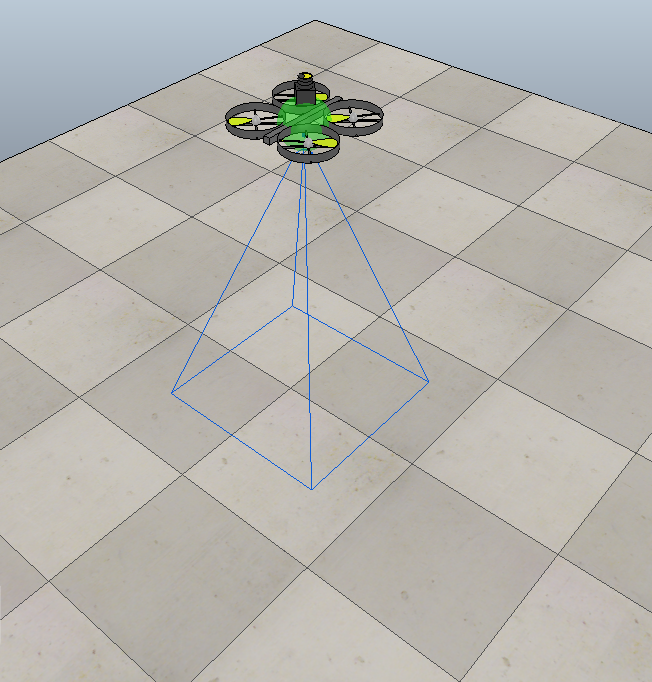
\includegraphics[width=0.23\textwidth]{figures/1m_height.png}}
%   \hfill
%   \subfigure[Big room]{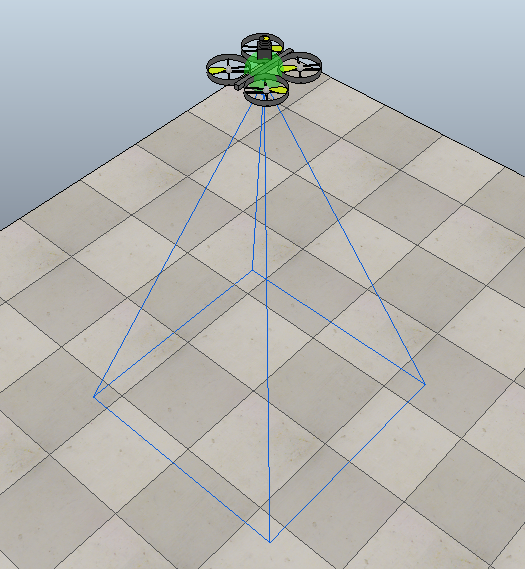
\includegraphics[width=0.23\textwidth]{figures/2m_height.png}}
  
%   \label{fig:2m_height}
%   \hfill
%   \subfigure[Big room]{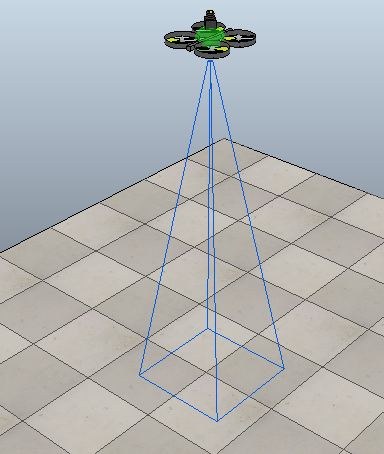
\includegraphics[width=0.23\textwidth]{figures/2m_height_small_clipping.png}}

%   \label{fig:2m_height}
  
%   \caption{Room Coverage}
% \end{figure}

% \begin{figure}[!htb]
% \minipage{0.32\textwidth}
%   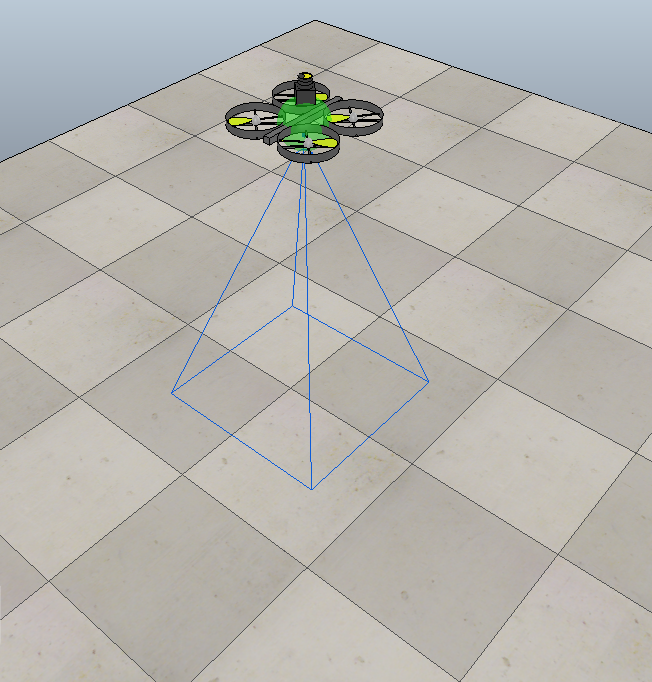
\includegraphics[width=\linewidth]{figures/1m_height.png}
%   \caption{A really Awesome Image}\label{fig:awesome_image1}
% \endminipage\hfill
% \minipage{0.32\textwidth}
%   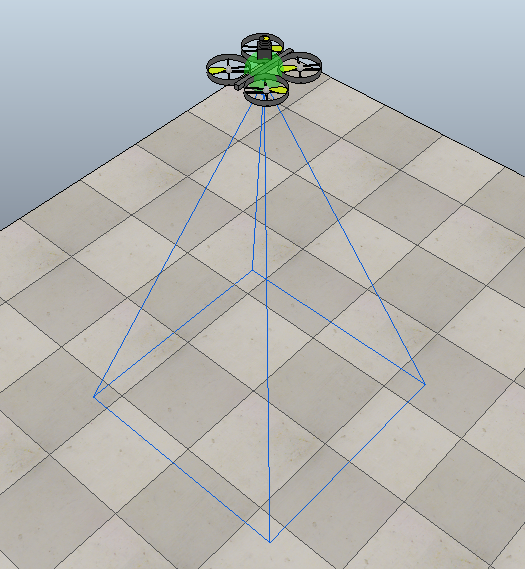
\includegraphics[width=\linewidth]{figures/2m_height.png}
% \endminipage\hfill
% \minipage{0.32\textwidth}%
%   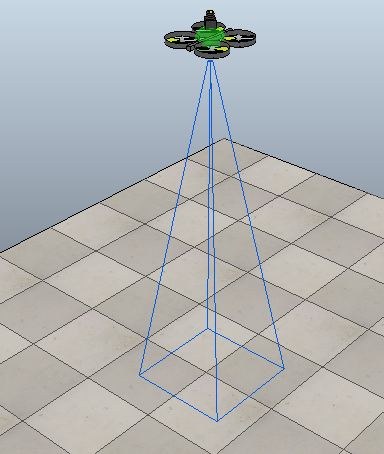
\includegraphics[width=\linewidth]{figures/2m_height_small_clipping.png}
% \endminipage
% \end{figure}

\textcolor{red}{CLEAN THE IMAGES TO BE OF THE SAME CONTOUR}

\begin{figure}[t]
\centering
\subfigure[text]{
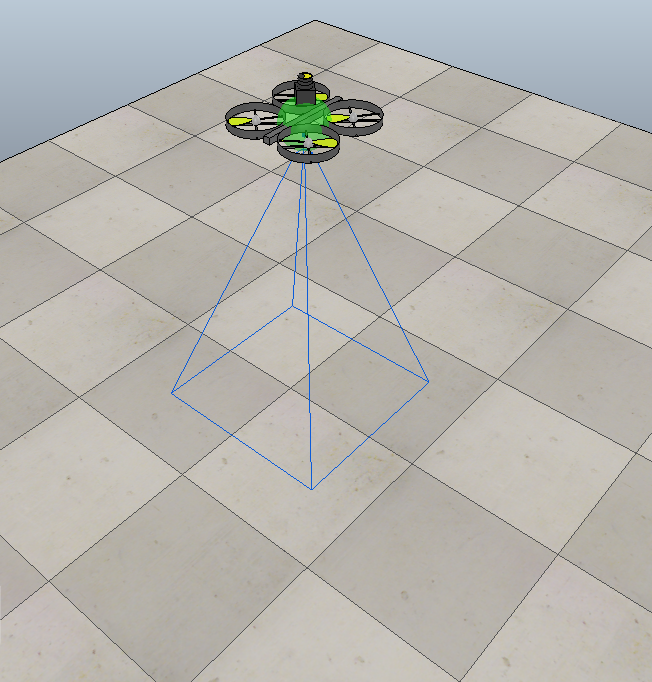
\includegraphics[width=.3\textwidth]{figures/1m_height.png}
}
\subfigure[text]{
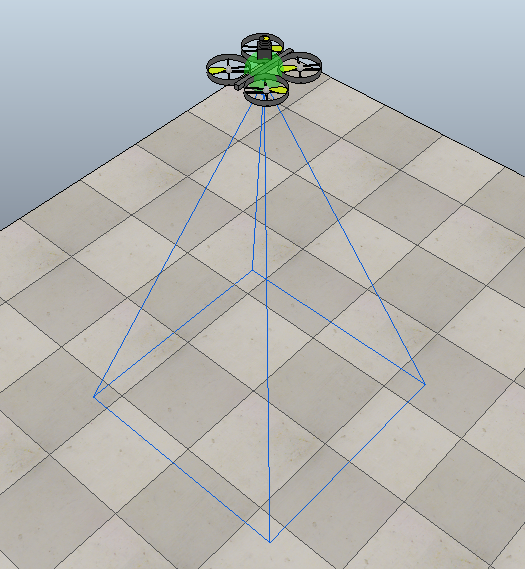
\includegraphics[width=.3\textwidth]{figures/2m_height.png}
}
\subfigure[text]{
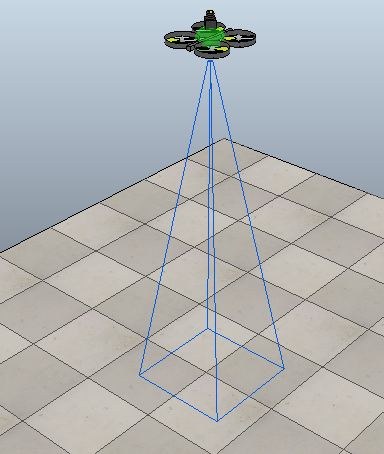
\includegraphics[width=.3\textwidth]{figures/2m_height_small_clipping.png}
}

\caption{blablabla}
\label{fig:whatever}
\end{figure}



\section{Real World Experiments} \label{real_robot}

\subsection{Quadcopter Hardware}\label{real_robot_hardware}

The Quadcoptor used to do this experiments is an offshelf commercially found drone from the French company Parrot which is AR.drone 2.0. It was first introduced in 2010 as a toy for Augmented Reality games. Shortly research labs, universities make use of its comparably cheap and low weight in their experiments. Hardware and software specification with sample research usage can be found in \cite{Ardrone1,Ardrone2}. Equipped with two cameras; one of them is pointing downwards makes it clearly very useful for the application of area coverage. This camera runs at 60 fps with a resolution of 176 x 144 pixels, covering a field of view of only 47.5$^{\circ}$ x 36.5$^{\circ}$. Concerning the software, there are mobile applications to control the drone for both IOS and Android. \textbf{SDK is avilable for computer} . The embedded software that is running onboard is not directly accessible, but sending and transmitting data with telnet shell communication channel is possible. Transmitting navigation data and receiving the sensor readings to the drone is done after connecting a workstation computer to it through ad-hoc wireless LAN network. External ROS packages used to control the quadcopter will be discussed in more details in the next subsections.


\subsection{Experiment Environment}

As mentioned in \ref{localization_Back} the wide scenarios of generating real experiments with aerial robots, localization problem is crucial. Using the monocular SLAM package developed for AR.Drone by Engel et al. in \cite{engel14ras,engel12iros}  is chosen to solve this challenge. This package proved by practical experimentation its reliability in localizing the robot without any environment modification except putting a panel full of figures to give rich features.

\textcolor{red}{put the image of the environment}


\subsection{Robot Localization }

The tum\_ardrone ROS package enables the drone to localize itself  and navigate in an unknown and potentially GPS-denied environments without learning the environment or mapping it previously. Monocular SLAM to compute a visual pose estimate within this map for each video frame. The main contribution of this package is to estimate the scale of map from inertial and altitude measurements by formulating the problem statistically, and deriving a closed-form solution for the maximum likelihood (ML) estimator of the unknown scaling factor. Proportional-integral-differential (PID) control is applied to control the pose of the drone, and fly to and hold a desired target position.


% Odometry Pose Estimation: The “Pose Estimator” is explained in the following article and Master’s Thesis [23], [22]. To correct the drift that the Odometry Pose Estimator module has, absolute measures provided by visual features are used.
 
\section{Mosaicking}
The ortho-mosaiced output image composed by the captured
images are very close to a complete top view of the area.
Mosaicing in our case is simply computed using the position and orientation coordinates of the known waypoint and stitch the images together to validate the optimum choice of the positions where the drone captured these images as shown in Fig.\ref{fig:final_room} for the simulated room in V-REP.

Otho-mosaicing also proved its validity in mosaicing aerial outdoor images as mentioned by Yahyanejad in  \cite{yahyanejad2010incremental}.

The coverage threshold rate is 90\% of the useful area in the room without taking the block parts into consideration to cover.
\hfill
\vfill

\begin{figure}[!tbp]
 \subfigure[Poses of every image captured in the room]{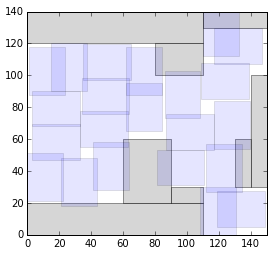
\includegraphics[width=0.45\textwidth]{figures/room_python.PNG}}
  \caption{Room Coverage}
\end{figure}

\hfill

\begin{figure}[!tbp]
  \centering
  \subfigure[Room mosaicing]{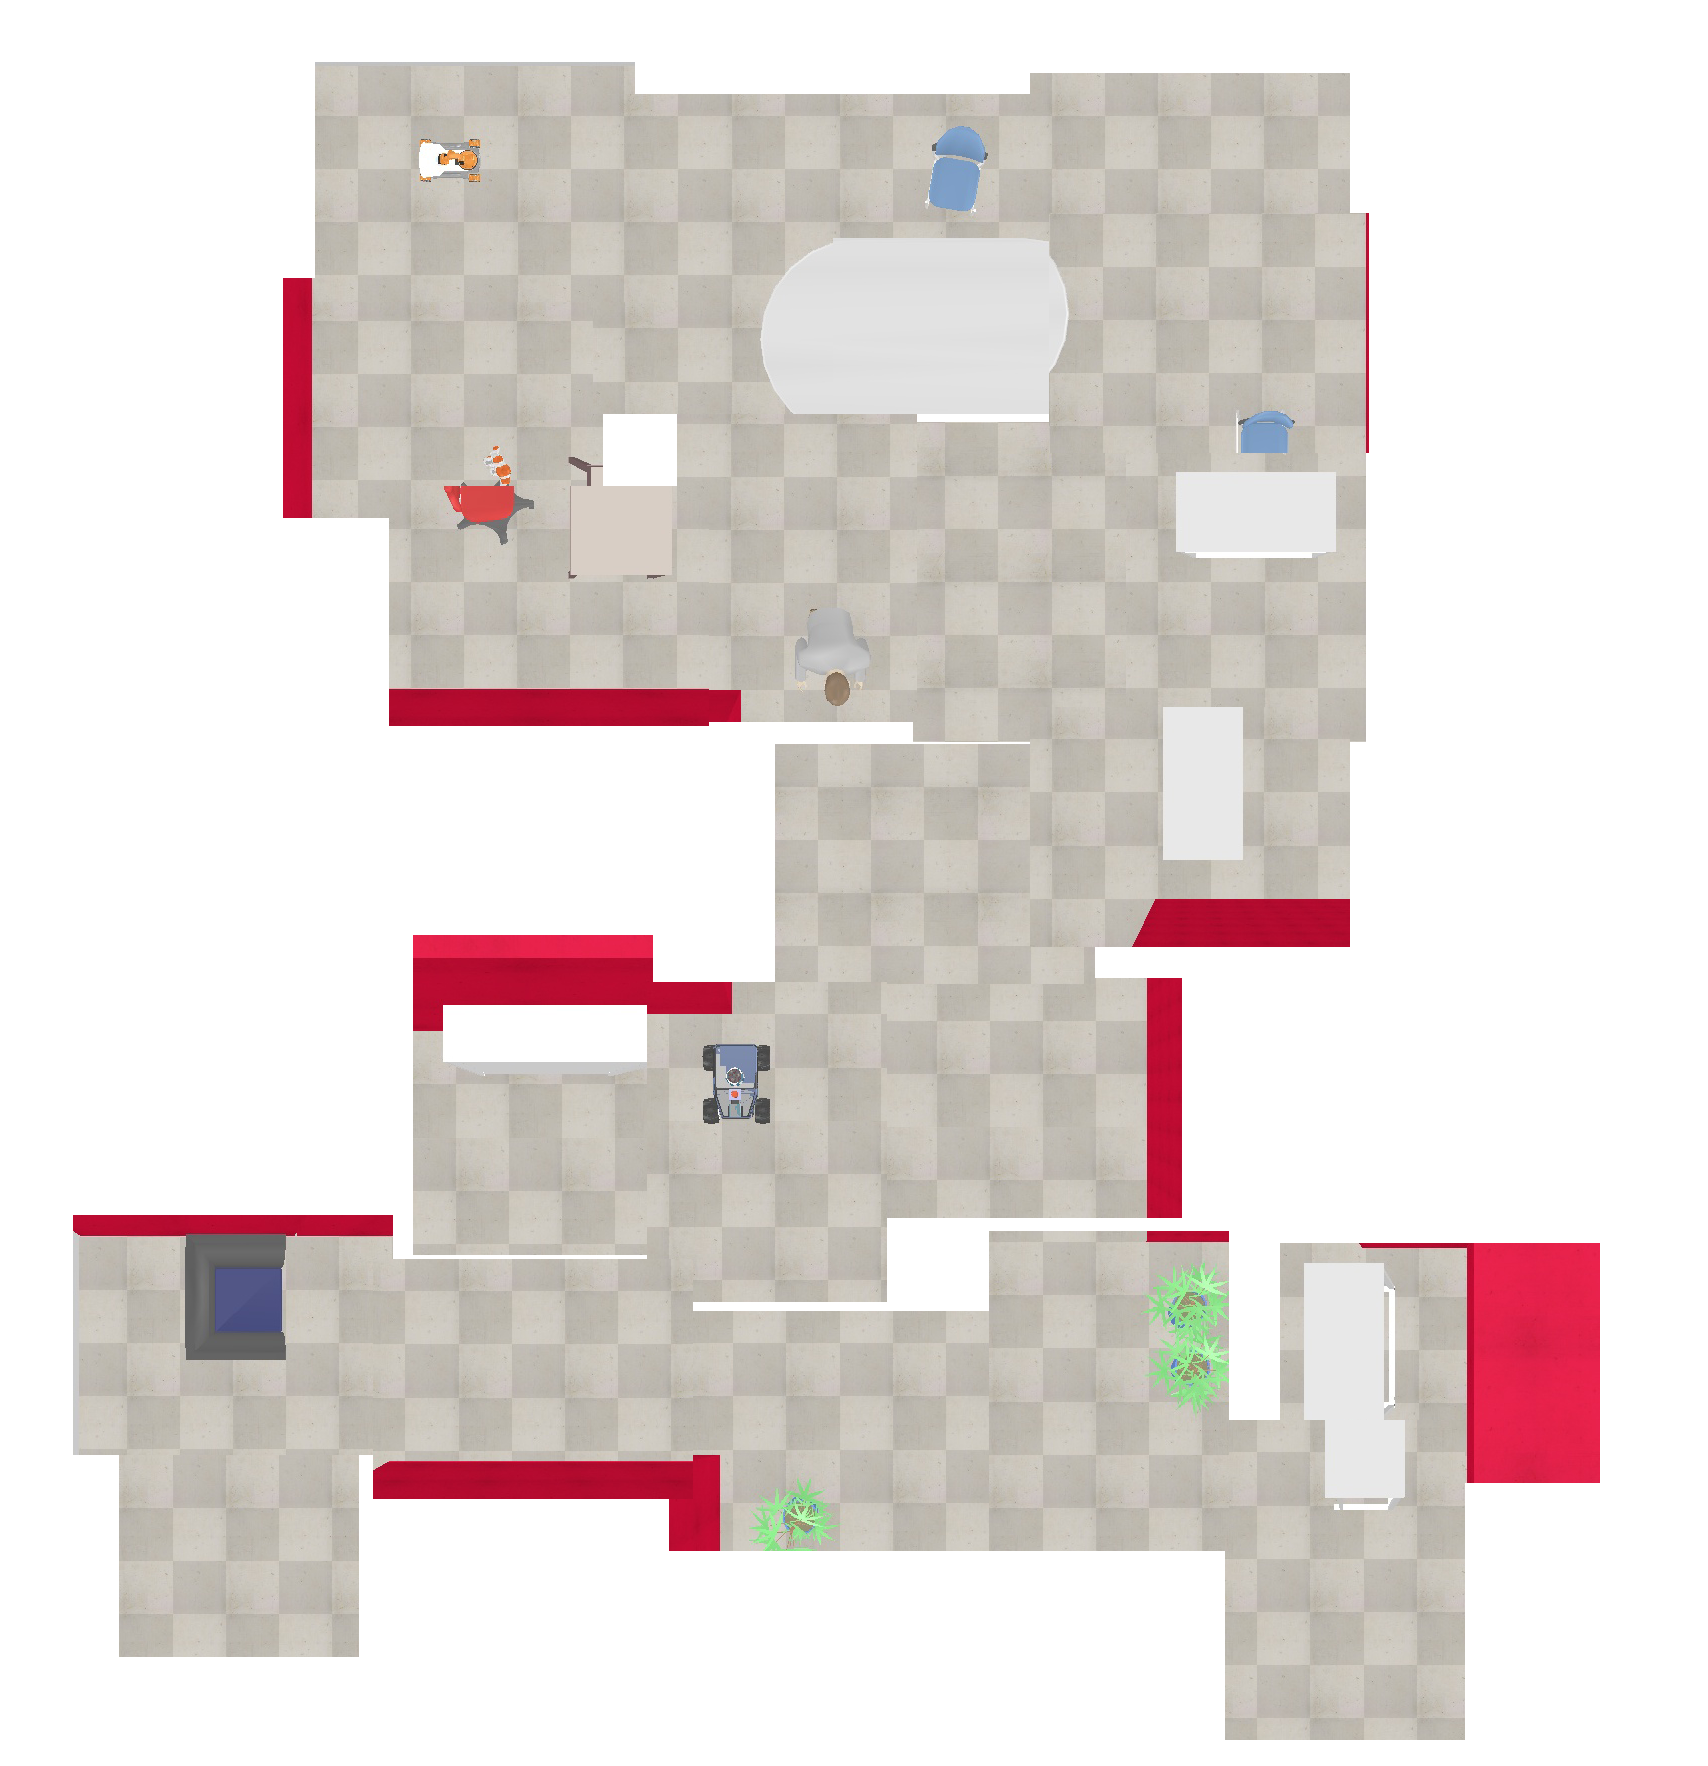
\includegraphics[width=0.45\textwidth]{figures/mosaic2.png}}
  \hfill
  \subfigure[Poses of every image captured in the room]{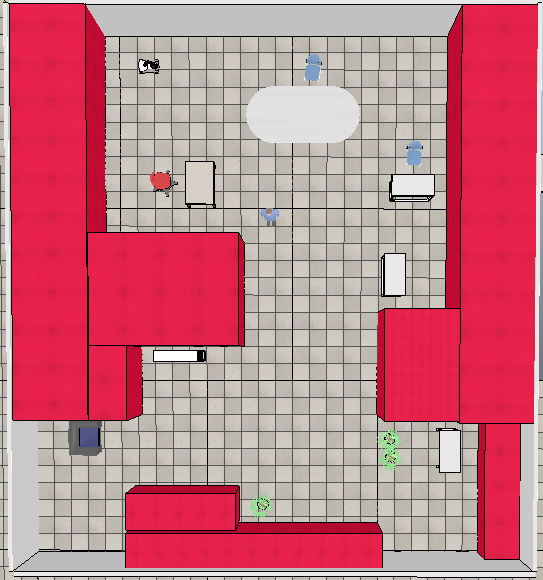
\includegraphics[width=0.45\textwidth]{figures/room_full.png}}
  \caption{Room Coverage}
  
  \label{fig:final_room}
  
\end{figure}

\hfill

\newpage

\section{Computation}
The computer used to generate these experiments is specified with 8 GB of memory (RAM). Processor is Intel® Core™ i7-2720QM CPU @ 2.20GHz ×8. 
The OS is ubuntu 14.04 LTS. Codes developed is developed by C++11, python 2, Matlab 2013B. V-REP version is 3.3.x. ROS Indigo is used.
\chapter{Conclusion} \label{chap:conc}

\section{Conclusion}
In this thesis, the coverage path planning is addressed with a new approach. This approach is dealing with area coverage problem as two different challenges. The first challenge is the optimized choice of poses that guarantee maximum area coverage. The second challenge is path planning of these chosen poses.

This thesis is considering nonregular areas. Evolutionary algorithms specifically genetic algorithm (GA) is used  and compared with other methods like particle swarm algorithm to solve the first problem of area coverage. GA approach efficiently cover 90\% of a given area. 

Several path planning approaches were tested. The design of having the multi layer of path planning is taken into account. Three algorithms were implemented,tested and compared results were presented. In all the three algorithms, there are two layers of path planning.  The first layer is formulating the robot poses as cities and connect them to form a graph which resembles the travelling sales man problem (TSP). GA is used to solve TSP and generate a list of poses of the cities that will insure least length of tour.

Then the second layer is different in the three algorithms. The first algorithm, takes the list of ranked poses and generate linear piecewise function linking all the poses. The second algorithm is using spline piecewise function instead of linear which generate smoother paths. Last but not least, the third approach, uses artificial potential field (APF) as the second layer of map representation and path planning. It is used mainly to avoid obstacles that appear on the map. Static obstacles are considered in this thesis. Efficiently traversing the map without the known falling in the trap of local minima.

One of the drawbacks of APF is the vast amount of parameter tuning needed before having the efficient results. This tuning is dependent on many factors like; a scaling factor of both the attractive and repulsive potentials, the current heading of the robot. It is also dependent on the shape of the map. The initial and final goal location being traversed are influencing the potential field too.

Some of the work presented in this thesis lead to a publication in URAI 2016 and will be presented in China on August 2016.

\section{Future Work}
\begin{itemize}
\item Impose dynamic obstacles in the map to validate the artificial potential field. 
\item Re-planning algorithms in real time can be tested.
\item RRT can be a good alternative to being tried instead of the artificial potential field.
\item The down camera of AR.Drone 2.0 is of low resolution. So thinking of attaching a camera to the drone and testing it will be of great importance for better results.
\end{itemize}


%\appendix
%\chapter{The first appendix}
If you need to add any appendix, do it here...
 Etc.
\chapter{Glossary}
UAV Unmanned Aerial Vehicle\\
ROS Robot Operating System \\
VTOL Vertical Take Off and Landing \\
AR Augmented Reality \\
IMU Inertial Measurement Unit\\
SLAM Simultaneous localization and mapping\\

\iffalse
AUV Autonomous Unmanned Vehicle \\
BSD Berkeley Software Distribution \\ 
∆ Amount of Increase \\
ESC Electronic Speed Controller\\
GPS Global Positioning System\\
κp Proportional Constant used in control\\
κi Integrative Constant used in control\\
κd Derivative Constant used in control\\
\Omega Angular Speed\\
\Phi Angular Speed in ¨ X direction\\
\psi Angular Speed in ¨ Z direction\\
PID Proportional-Integral-Derivative controller\\

UWV Unmanned Water Vehicle\\
\theta Angular Speed in ¨ Y direction\\

\fi

%   this is for BibTeX.  remove if you plan to write the references in the document
\bibliographystyle{plain}
\bibliography{refs}


%adds the bibliography to the table of contents
\addcontentsline{toc}{chapter}
         {\protect\numberline{Bibliography\hspace{-96pt}}}

\end{document}
